\section{GUI - Package Structure}
\begin{figure}[!ht]
\begin{center}
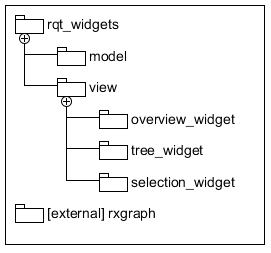
\includegraphics[scale=1.0]{./bilder/package_structure_gui.png}
\caption{The package structure of the GUI}
\label{The package structure of the GUI}
\end{center}
\end{figure}

\mbox{}

\newpage


\section{GUI - Model}
\begin{figure}[!ht]
\begin{center}
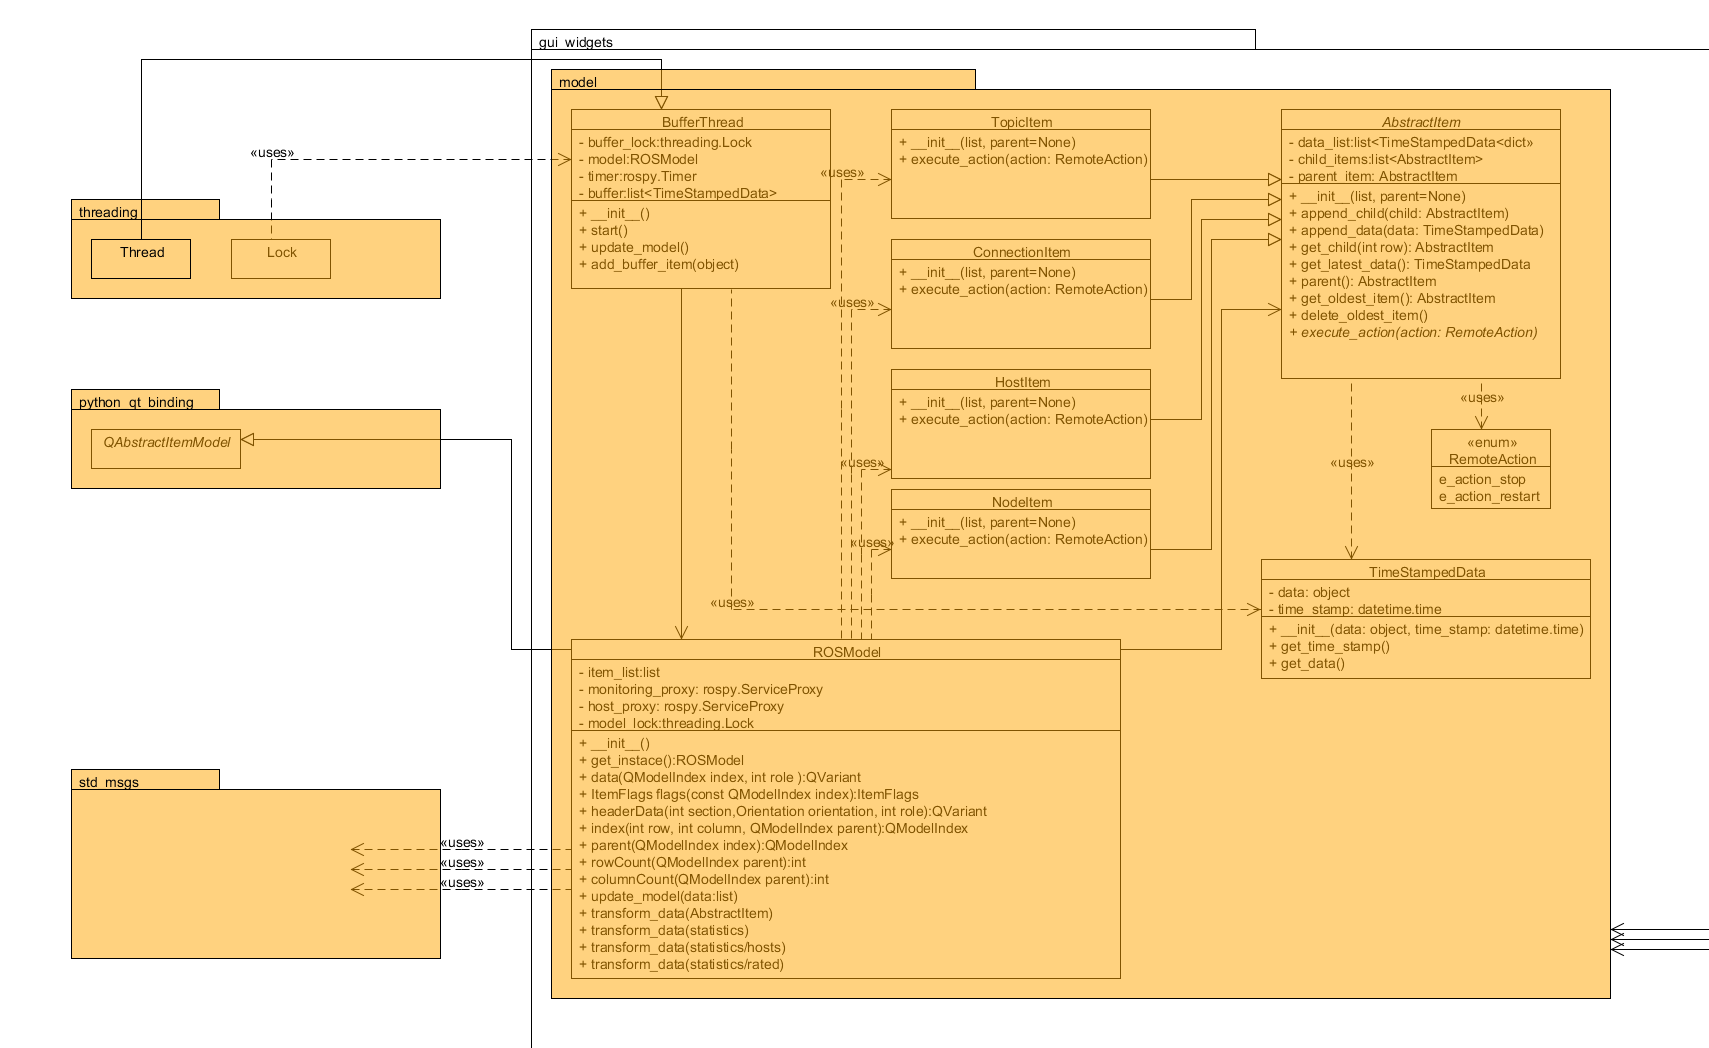
\includegraphics[width=1.0\linewidth]{./bilder/model.png}
\caption{The model class diagram}
\end{center}
\end{figure}

\subsection{BufferThread}
This thread should buffer the incoming data from the topics and regulary update the model.
\subsubsection{Attributes}
\begin{itemize}
  \item \textbf{private buffer\_lock: threading.Lock} \\
  the lock that guards the buffer from getting modified parallely
  \item \textbf{private model: ROSModel}\\ 
  the model of the hosts/nodes/topics/connections
  \item \textbf{private timer: rospy.Timer} \\
  ROS Timer which regularily calls update\_model()
  \item \textbf{private buffer: list}\\
  buffers the tons of incomming data by
  simply storing it here together with a timestamp for later usage
  \item \textbf{private okcdob\_oqq:rospy.OkcdobOqq}\\ 
  Drsc sc kx okcdob oqq. Myxqbkdevkdsyxc.
  \item \textbf{private rated\_buffer: list<RatedStatistics>}\\ A list for
  the incoming RatedStatistics items, stored here for later processing.
\end{itemize}
\subsubsection{Methods}
\begin{itemize}
%  \item \textbf{public \_\_init\_\_()} 
  \item \textbf{public start()}\\
  starts the thread and also the timer for regulary updates of the model
  \item \textbf{public update\_model()}\\ 
  starts the update of the model. Will be called regulary by the timer.
  \item \textbf{public add\_buffer\_item(object)}\\ 
  adds an item to the buffer list. Will be called whenever data from the topics
  is available.
  \item \textbf{public add\_buffer\_item(RatedStatistics)}\\
  adds an RatedStatistics item to the rated\_buffer
\end{itemize}

\subsection{ROSModel}
Represents the data as a QtModel. This enables automated updates of the View.
\subsubsection{Attributes}
\begin{itemize}
 % \item \textbf{private item\_list: list}
  \item \textbf{private monitoring\_proxy: rospy.ServiceProxy}\\ 
  the proxy to the monitoring node for obtaining statistics and rated statistics of the past minutes. To be called only once when the GUI started and the MonitoringNode has been running for a while
  \item \textbf{private model\_lock: threading.Lock}\\ 
  protects the model from parallel modification
  \item \textbf{private log: list<list<string>>}\\ 
  global log of all the events having occured in the past  
  \item \textbf{private root\_item: AbstractItem}\\
  contains the list of headers
  \item \textbf{private item\_delegate: SizeDelegate}\\
  
  \item \textbf{private log\_model: QStandardItemModel}\\
   
\end{itemize}
\subsubsection{Methods}
\begin{itemize}
  \item \textbf{public \_\_init\_\_()}\\ 
  defines the class attributes especially the root\_item which later contains the list of headers e.g. for a TreeView representation
  \item \textbf{public ROSModel get\_instance()}\\
  returns the instance of the ROSModel
  \item \textbf{public list<list<string>> get\_log()}\\
  returns the global log-file as a list
  \item \textbf{public QVariant data(index:QModelIndex, role:int)}\\
  returns the data of an item at the given index
  \item \textbf{public ItemFlags flags(index:QModelIndex)}\\
  returns the flags of the item at the given index (like Qt::ItemIsEnabled)
  \item \textbf{public QVariant headerData(section:int, orientation:Orientation,
  role:int)}\\ 
  returns the headerData  at the given section
  \item \textbf{public QModelIndex index(row:int, column:int,
  parent:QModelIndex)}\\
  returns the index of an item at the given column/row
  \item \textbf{public QModelIndex parent(index:QModelIndex)}\\ 
  returns the QModelIndex of the parent of the child item specified via its index
  \item \textbf{public int rowCount(QModelIndex)}\\ 
  returns the amount of rows in the model
  \item \textbf{public int columnCount(QModelIndex)}\\
  returns the amount of columns in the model
  \item \textbf{public update\_model(data:list)}\\ 
  updates the model by using the items of the list. The items will be of the message types 
  \item \textbf{public transform\_data(AbstractItem)}\\ 
  integrates a TopicStatistics in the model by modifing its item/s by adding a new dict to the corresponding item (especially the TopicItem and the ConnectionItem)
  \item \textbf{public transform\_data(statistics)}\\ 
  integrates a NodeStatistics in the model by modifing its item/s by adding a new dict with the entries of the given parameter
  \item \textbf{public transform\_data(HostStatistics)}\\ 
  integrates a HostStatistics in the model by modifing its item/s by adding a new dict with the entries of the given parameter
  \item \textbf{public transform\_data(RatedStatistics)}\\ 
  add the rating to an existing entry by modifing the dict of the corresponding
  item/s
  \item \textbf{public transform\_data(StatisticHistory)}\\ 
  When using the monitor\_proxy to receive about the last minutes from the monitoring node
  it returns a StaticHistory item which can then be integrated in the model via this method
  \item \textbf{public void trigger\_node\_action(string, RemoteAction)}\\
  triggers the RemoteAction to start,stop or restart a node
  \item\textbf{public void add\_log\_item(list<string>)}\\
  adds the given lists as a log entry to the model
  \end{itemize}

\subsection{AbstractItem}
Provides a unified interface to access the items of a model.
\subsubsection{Attributes}
\begin{itemize}
  \item \textbf{private data\_list: list<dict>}\\ 
  contains the data of the abstract item including a time stamp so that
  the progress in time can be shown
  \item \textbf{private child\_items: list<AbstractItem>}\\ 
  the child of this item
  \item \textbf{private parent\_item: AbstractItem}\\ 
  the parent of this item
  \item \textbf{private log: list<list<string>>}\\
  contains the logs of the item
\end{itemize}
\subsubsection{Methods}
\begin{itemize}
%  \item \textbf{public \_\_init(list, parent=None)\_\_}
   \item \textbf{public void append\_child(AbstractItem)}\\ 
   append a child to the list of childs
  \item \textbf{public void append\_data(oject)}\\ 
  append data to the data\_list of the AbstractItem
  \item \textbf{public AbstractItem get\_child(row: int)}\\ 
  return the child at the position row
  \item \textbf{public object get\_latest\_data()}\\ 
  return the latest data of the data\_list
  \item \textbf{public AbstractItem parent()}\\ 
  returns the parent of this or None if there is none (TODO:is that correct)
  \item \textbf{public AbsractItem get\_items\_older\_than(rospy.Time)}\\
  returns all items wich are older than \textit{rospy.Time}
  \item \textbf{public void delete\_items\_older\_than(rospy.Time})\\
  deletes all items wich are older than \textit{rospy.Time}
  \item \textbf{public AbstractItem get\_items\_younger\_than(rospy.Time)}\\
  returns all items wich are younger than \textit{rospy.Time}
  \item \textbf{public abstract void execute\_action(RemoteAction)}\\ 
  executes a action on the current item like stop or restart. Calls to this
  method should be redirected to the remote host on executed there.
\end{itemize}

\subsection{HostItem}
A HostItem represents a host with all its data.
The data\_list will contain TimeStampedData whereas the data is a dict
containing ...
\subsubsection{Methods}
\begin{itemize}
%  \item \textbf{public \_\_init(list, parent=None)\_\_}
  \item \textbf{public execute\_action(RemoteAction)}\\
  sends a signal to stop or restart a node
\end{itemize}

\subsection{NodeItem}
 A NodeItem represents a node with all of its data. It also has a interface to start/stop/restart nodes.
 The data\_list will contain TimeStampedData whereas the data is a dict containing ...
\subsubsection{Methods}
\begin{itemize}
 % \item \textbf{public \_\_init(list, parent=None)\_\_}
  \item \textbf{public execute\_action(RemoteAction)}\\
  sends a signal to stop or restart the node
\end{itemize}

\subsection{TopicItem}
A ConnectionItem reprensents the connection between a publisher and a subscriber and the topic they are puglishing / listenening on.
The data\_list will contain TimeStampedData whereas the data is a dict containing ...
\subsubsection{Methods}
\begin{itemize}
%  \item \textbf{public \_\_init(list, parent=None)\_\_}
  \item \textbf{public execute\_action(RemoteAction)}\\ 
  not senseful, throws an exception
\end{itemize}

\subsection{ConnectionItem}
 A NodeItem represents a node with all of its data. It also has a interface to start/stop/restart nodes.
 The data\_list will contain TimeStampedData whereas the data is a dict containing ...
\subsubsection{Methods}
\begin{itemize}
%  \item \textbf{public \_\_init(list, parent=None)\_\_}
  \item \textbf{public execute\_action(RemoteAction)}\\ 
  not senseful, throws an exception
\end{itemize}

% \subsection{TimeStampedData}
% ..
% \subsubsection{Attributes}
% \begin{itemize}
%   \item \textbf{private data: object}
%   ..
%   \item \textbf{private time\_stamp: datetime.time}
%   ..
% \end{itemize}
% \subsubsection{Methods}
% \begin{itemize}
%   \item \textbf{public \_\_init(object, datetime.time)\_\_}
%   ..
%   \item \textbf{public datetime.time get\_time\_stamp()}
%   ..
%   \item \textbf{public object get\_data()}
%   ..
% \end{itemize}

\subsection{Enum RemoteAction}
Gives a predefinition for a remote interaction with hosts and nodes.
\subsubsection{Types}
\begin{itemize}
	\item \textbf{e\_action\_stop}\\
	the action that should stop a host or node
	\item \textbf{e\_action\_restart}\\
	the action that should restart a host or node
\end{itemize}

\subsection{ItemFilterProxy}
TODO:Description
\subsection{Attributes}
\begin{itemize}
  \item \textbf{private show\_hosts: bool}\\
  true if show\_hosts\_check\_box is selected
  \item \textbf{private show\_nodes: bool}\\
  true if show\_nodes\_check\_box is selected
  \item \textbf{private show\_connections}\\
  true if show\_connections\_check\_box is selected
  \item \textbf{private show\_topics: bool}\\
  true if show\_topics\_check\_box is selected
\end{itemize}
\subsubsection{Methods}
\begin{itemize}
  %??
  %\item \textbf{public void \_\_init\_\_(QObject)}\\
  
  \item \textbf{public ItemFilterProxy get\_instance()}\\
  returns the instance of the Proxy
  \item \textbf{public bool filterAcceptsRow(int, QModelIndex)}\\
  
  \item \textbf{public bool lessThan(QModelIndex, QModelIndex)}\\
  
  \item \textbf{public void show\_hosts()}\\
  
  \item \textbf{public void show\_nodes()}\\
  
  \item \textbf{public void show\_connections()}\\
  
  \item \textbf{public void show\_topics()}\\
  
\end{itemize}

\subsection{LogFilterProxy}
TODO:Description
\subsection{Attributes}
\begin{itemize}
  \item \textbf{private current\_item: AbstractItem}\\
  the currently selected item
\end{itemize}
\subsubsection{Methods}
\begin{itemize}
  %??
  %\item \textbf{public void \_\_init\_\_(QObject)}\\
  
  \item \textbf{public ItemFilterProxy get\_instance()}\\
  returns the instance of ItemFilterProxy
  \item \textbf{public bool filterAcceptsRow(int, QModelIndex)}\\
  
  \item \textbf{public bool lessThan(QModelIndex, QModelIndex)}\\
  
  \item \textbf{public void filter\_by\_item(AbstractItem)}\\
  filters the content by AbstractItem
\end{itemize}

\subsection{SizeDelegate: QtGui.QStyledItemDelegate}
Makes it possible to change the font size of the Gui-Plugin content
\subsubsection{Attributes}
\begin{itemize}
  \item \textbf{private current\_font\_size: int}\\
  the size displayed font
\end{itemize}
\subsubsection{Methods}
\begin{itemize}
  \item \textbf{public void paint(QPainter, QStyleOptionViewItem,
  QModelIndex)}\\
  paints the font
  \item \textbf{public void set\_bigger\_font\_size()}\\
  increases the displayed font-size
  \item \textbf{public void set\_smaller\_font\_size()}\\
  decreases the displayed font-size
\end{itemize}

\newpage
\section{GUI - View}
\begin{figure}[!ht]
\begin{center}
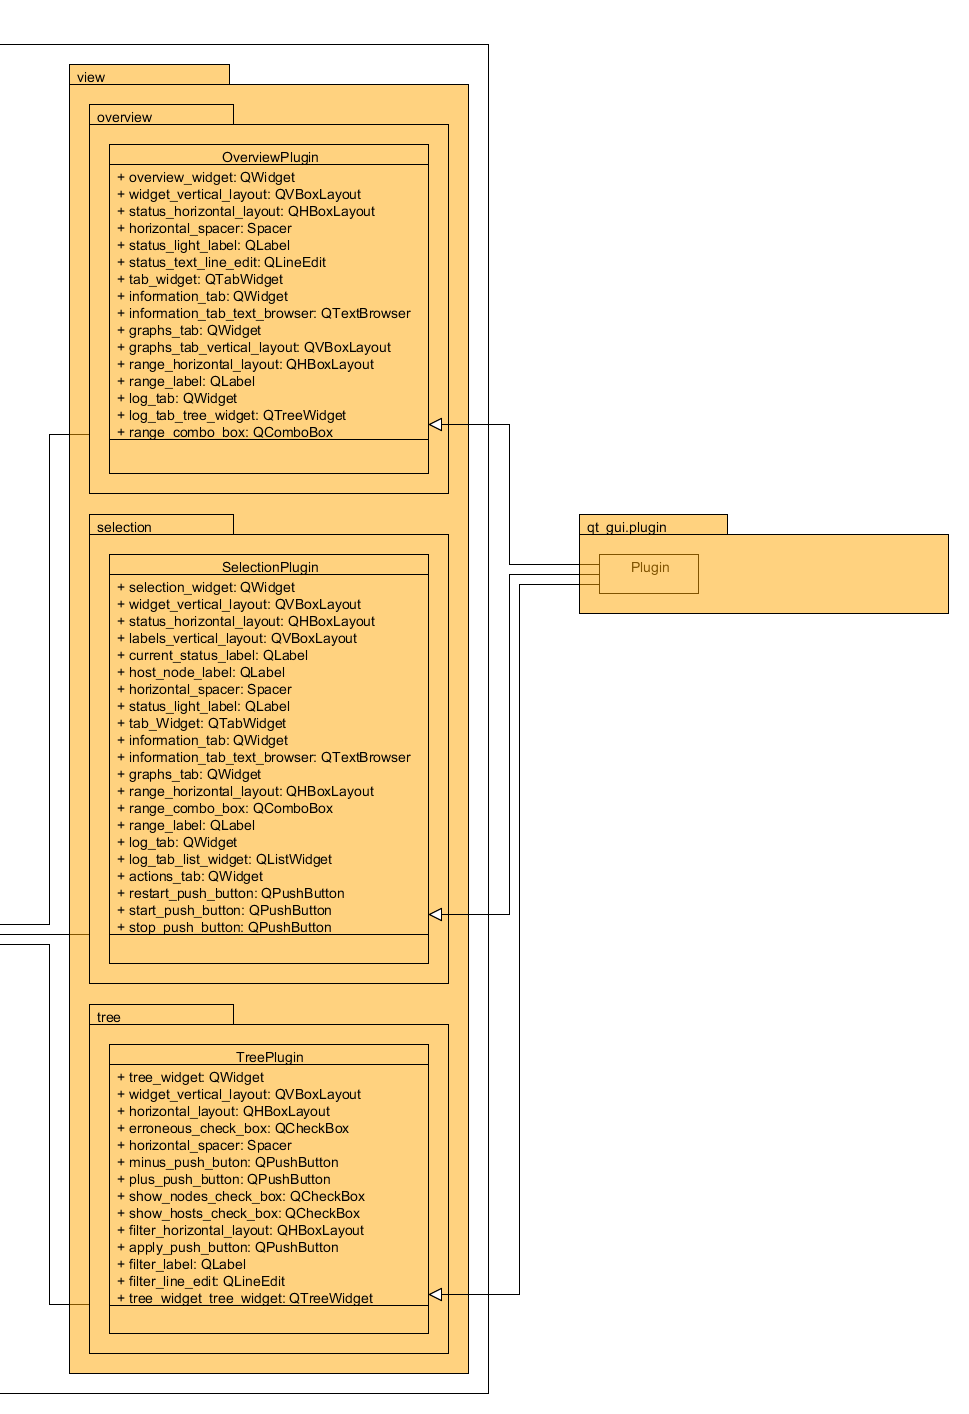
\includegraphics[width=0.8\linewidth]{./bilder/view.png}
\caption{The view class diagram}
\end{center}
\end{figure}

\subsection{OverviewPlugin}
The OverviewPlugin is the core of the graphical user interface, which
contains most of the relevant information in a small and fancy area.
\subsubsection{Attributes}
\begin{itemize}
  \item \textbf{public overview\_widget: QWidget}\\
  the object wich holds the widget
  \item \textbf{public status\_light\_label: QLabel}\\
  a status ligth wich shows if everything is ok or not
  \item \textbf{public tab\_widget: QTabWidget}\\
  the object wich holds the different tabs of the widget
  \item \textbf{public information\_tab: QWidget}\\
  a tab wich gives general information about the network 
  \item \textbf{public graphs\_tab: QWidget}\\
  displays graphs about the network
  \item \textbf{public range\_combo\_box: QComboBox}\\
  makes it possible to set the range of the graphs
  \item \textbf{public log\_tab: QWidget}\\
  shows actual errors and warnings
  \item \textbf{public draw\_graphs: bool}\\
  when the graph tab is selected, draw\_graphs is set on true an the graph will
  appear
  \item \textbf{public last\_update: rospy.Time}\\
  the time of the latest update
  \item \textbf{public graph\_layout: pyqtgraph.GraphicsLayoutWidget}\\
  
  \item \textbf{public graph\_dict: dict<string, pyqtgraph.PlotItem>}\\
  
  \item \textbf{public values\_dict: dict<string, numpy.ndarray>}\\
  
  \item \textbf{public model: ROSModel}\\
  
  \item \textbf{public log\_fiter\_proxy: LogFilterProxy}\\
  
\end{itemize}
\subsubsection{Methods}
\begin{itemize}
%   \item \textbf{public void \_\_init\_\_(context)}\\
%   ..
  \item \textbf{public void connect\_slots()}\\
  initializes the slots from the widget
  \item \textbf{public void update()}\\
  updates the widget
  \item \textbf{public void on\_current\_tab\_changed(int)}\\
  
  \item \textbf{public void update\_graphs()}\\
  
\end{itemize}

\subsection{TreePlugin}
TreePlugin is very simply and shows only the actual active hosts
and nodes. It is possible to filter the output, e.g. only erroneus hosts or
nodes are displayed.
\subsubsection{Attributes}
\begin{itemize}
  \item \textbf{public tree\_widget: QWidget}\\
  the object wich holds the widget
  \item \textbf{public erroneous\_check\_box: QCheckBox}\\
  only erroneous hosts and nodes will be displayed
  \item \textbf{public show\_node\_check\_box: QCheckBox}\\
  displays the activ nodes
  \item \textbf{public show\_host\_check\_box: QCheckBox}\\
  displays the activ hosts
  \item \textbf{public show\_topics\_check\_box: QCheckBox}\\
  displays the actual topics
  \item \textbf{pubic show\_connects\_check\_box: QCheckBox}\\
  displays the actual connections
  \item \textbf{public plus\_push\_button: QPushButton}\\
  makes it for, a better clarity, possible to zoom in  
  \item \textbf{public minus\_push\_button: QPushButton}\\
  and zoom out
  \item \textbf{public selection\_widget: SelectionWidget}\\
  the object of the SelectionWidget
  \item \textbf{public filter\_line\_edit: QLineEdit}\\
  a textfield where you can define a filter for the output
  \item \textbf{public model: ROSModel}\\
  the connection to the ROSModel
  \item \textbf{public filter\_proxy: ItemFilterProxy}\\
  
  \item \textbf{public size\_delegate: SizeDelegte}\\
  
\end{itemize}
\subsubsection{Methods}
\begin{itemize}
%   \item \textbf{public void \_\_init\_\_(context)}\\
%   ..
  \item \textbf{public void connect\_slots()}\\
  initializes the slots from the widget
  \item \textbf{public void on\_show\_nodes\_check\_box\_state\_changed()}\\
  displays or delete the nodes in the box wether the check box is set or unset
  \item \textbf{public void on\_show\_hosts\_check\_box\_state\_changed()}\\
  displays or delete the host in the box wether the check box is set or unset
  \item \textbf{public void on\_show\_topics\_check\_box\_state\_changed()}\\
  displays or delete the topics in the box wether the check box is set or unset
  \item \textbf{public void
  on\_show\_connections\_check\_box\_state\_changed()}\\
  displays or delete the connections in the box wether the check box is set or
  unset
  \item \textbf{public void on\_apply\_push\_button\_clicked()}\\
  filters the content in the box according to the content of the
  filter\_line\_edit
  \item \textbf{public void on\_erroneus\_check\_box\_state\_changed()}\\
  if this check box is set, only erroneus hosts and nodes will be displayed  
  \item \textbf{public void on\_plus\_push\_button\_clicked()}\\
  checks if the plus\_push\_button is clicked and zoomes in (increases the size
  of the font)
  \item \textbf{public void on\_minus\_push\_button\_clicked()}\\
  checks if the minus\_push\_button is clicked and zoomes out (decreases the
  size of the font)
  \item \textbf{public void on\_item\_in\_tree\_view\_double\_clicked()}\\
  handels the double-click action and opens the clicked host or node in the
  SelectionWidget
\end{itemize}

\subsection{SelectionWidget}
A Widget wich is a part of the TreePlugin. It shows detailed information
in different tabs about the currently selected host or node.
\subsubsection{Attributes}
\begin{itemize}
  \item \textbf{public selection\_widget: QWidget}\\
  the object wich holds the widget
  \item \textbf{public host\_node\_label: QLabel}\\
  the name of the actual selected host or node
  \item \textbf{public status\_light\_label: QLabel}\\
  a status-light about the status of the current host or node
  \item \textbf{public tab\_widget: QTabWidget}\\
  the object wich holds the different tabs of the widget
  \item \textbf{public information\_tab: QWidget}\\
  a tab wich gives general information about hosts or nodes 
  \item \textbf{public graphs\_tab: QWidget}\\
  displays graphs about the actual selected host or node, e.g the Network- and
  CPU-Load
  \item \textbf{public range\_combo\_box: QComboBox}\\
  makes it possible to set the range of the graphs
  \item \textbf{public log\_tab: QWidget}\\
  shows actual errors and warnings
  \item \textbf{public actions\_tab: QWidget}\\
  includes buttons to restart and stop nodes
  \item \textbf{public selected\_item: item}\\
  the selected item
  \item \textbf{public draw\_graphs: bool}\\
  when the graph tab is selected, draw\_graphs is set on true an the graph will
  appear
  \item \textbf{public last\_updated: rospy.Time}\\
  the time of the last update
  \item \textbf{public graph\_layout: pygraph.GraphicsLayoutWidget}\\
  
  \item \textbf{public graph\_dict: dict<string, pyqtgraph.PlotItem>}\\
  
  \item \textbf{public values\_dict: dict<tring, numpy.ndarray}\\
  
  \item \textbf{public model: ROSModel}\\
  the connection to the RPSModel
  \item \textbf{public log\_filter\_proxy: LogFilterProxy}\\
  
\end{itemize}
\subsubsection{Methods}
\begin{itemize}
%   \item \textbf{public void \_\_init\_\_(context)}\\
%   ..
  \item \textbf{public void connect\_slots()}\\
  initializes the slots from the widget
  \item \textbf{public void set\_selected\_item(item)}\\
  set the selected item
  \item \textbf{public void update()}\\
  updates the widget
  \item \textbf{public void on\_current\_tab\_changed(int)}\\
  will call when the you switch between tabs
  \item \textbf{public void on\_restart\_push\_button\_clicked()}\\
  handels the retart button and restarts a host or node
  \item \textbf{public void on\_stop\_push\_button\_clicked()}\\
  handels the stop button and stops a host or node
  \item \textbf{public void on\_start\_push\_button\_clicked()}\\
  handels the start button and starts ahost or node
  \item \textbf{public void on\_range\_combo\_box\_index\_changed(int)}\\
  handels the change of the graph range
  \item \textbf{public void on\_changed\_selected\_item(QModelIndex)}\\
  handels the change of the selected item
  \item \textbf{public void update\_graphs()}\\
  updates the graph plot
\end{itemize}



